% !TEX program = xelatex
%
% Build:
%   xelatex slides-en.tex
%   xelatex slides-en.tex

\documentclass[aspectratio=169,10pt]{beamer}

\usetheme[progressbar=frametitle,numbering=fraction]{metropolis}
\usepackage{booktabs}
\usepackage{amsmath,amssymb}
\usepackage{xcolor}
\usepackage{tikz}
\usetikzlibrary{arrows.meta,positioning,fit,backgrounds}
\usepackage{graphicx}
\graphicspath{{figures/}}

\definecolor{mDarkTeal}{HTML}{23373B}
\definecolor{mLightBrown}{HTML}{EB811B}
\definecolor{mLightGreen}{HTML}{14B03D}
\setbeamercolor{alerted text}{fg=mLightBrown}

\title{From Three-Layer Corruption to Forget-Set Audit\\ in LLM Unlearning}
\subtitle{No unlearn runs --- forget-set geometry alone gives rank-level side-effect warnings}
\date{}
\author{Bo \;|\; \texttt{unlearning/}}
\institute{Llama-3.1-8B-Instruct \;+\; GradAscent \;+\; WikiText-103 (HDBSCAN $\times$ 10)}

\begin{document}

\maketitle

% ────────────────────────────────────────────────────────────────────────────
\section{Problem \& setup}

\begin{frame}{Research problem: unlearning hurts unrelated data}
    \textbf{Context.}\;
    Copyright / privacy / toxic content $\Rightarrow$ legal \& ethical demand to
    \emph{selectively delete} specific training data from an LLM $\Rightarrow$
    \textbf{LLM unlearning}.

    \vspace{0.5em}
    \textbf{But unlearning is not surgical.}
    Forgetting $\mathcal{D}_f$ \textbf{simultaneously damages} knowledge unrelated to $\mathcal{D}_f$ ---
    we call this \alert{knowledge corruption}; its radius and consequences are not yet characterised.

    \vspace{0.5em}
    \textbf{Benchmarking pain point.}
    Studying this \emph{systematically} --- establishing the pattern and comparing
    100 candidate forget sets --- needs $N$ unlearn runs + an $N \!\times\! N$ cross-PPL matrix.
    Cost scales quadratically; our $N=100$ already takes several GPU-hours.

    \vspace{0.8em}
    \begin{center}
        \large
        \alert{How can we \textbf{cheaply and systematically} assess the corruption a forget set will cause?}
    \end{center}
\end{frame}

\begin{frame}{Experimental setup: triplet schema + cross-eval matrix}
    \textbf{Data.} WikiText-103 $\to$ HDBSCAN clustered into \textbf{10 semantic clusters}
    \scriptsize(Federer / Harry Potter / tennis-match / \dots)\small.

    \vspace{0.4em}
    \textbf{Triplet schema} --- 10 triplets per cluster, \textbf{100 total}:
    \begin{center}
    \footnotesize
    \begin{tabular}{@{}lll@{}}
        \toprule
        split & 50 texts & downstream use \\
        \midrule
        \texttt{train}      & \textbf{forget set} $\mathcal{D}_f$   & fed to unlearn (GradAscent) \\
        \texttt{validation} & retain neighbours (same cluster)      & retain-side loss + L2 probe \\
        \texttt{test}       & probe samples (same cluster)          & L2 / L3 evaluation \\
        \bottomrule
    \end{tabular}
    \end{center}
    \small
    Three splits \emph{in the same cluster but mutually disjoint} $\Rightarrow$ naturally measure three semantic distances.

    \vspace{0.4em}
    \textbf{Evaluation.} Every ckpt is evaluated (PPL) on \emph{every other} triplet
    $\Rightarrow$ $N \!\times\! N$ cross-matrix $\Rightarrow$ diagonal / off-diagonal
    $\Rightarrow$ L1 / L2 / L3.
\end{frame}

% ────────────────────────────────────────────────────────────────────────────
\begin{frame}{One-sentence contribution}
    \begin{center}
        \large
        Unlearning side-effects \textbf{decay across three layers --- but never reach zero}.
    \end{center}

    \vspace{0.8em}
    \begin{center}
        \Large
        \textbf{L1 \;1.96$\times$} \;$\to$\; \textbf{L2 \;1.32$\times$} \;$\to$\; \textbf{L3 \;1.19$\times$}
    \end{center}

    \vspace{0.8em}
    \begin{center}
        \normalsize
        And \alert{73.8\,\%} of ``irrelevant'' samples still see elevated PPL.
    \end{center}

    \vfill
    \footnotesize\itshape\centering
    Llama-3.1-8B-Instruct $\cdot$ GradAscent $\cdot$ $n=100$ forget sets (10 HDBSCAN clusters $\times$ 10).
\end{frame}

% ────────────────────────────────────────────────────────────────────────────
\section{Definitions}

\begin{frame}{Three layers + how we quantify}
    \begin{columns}[T,onlytextwidth]
    \column{0.56\textwidth}
    \centering
    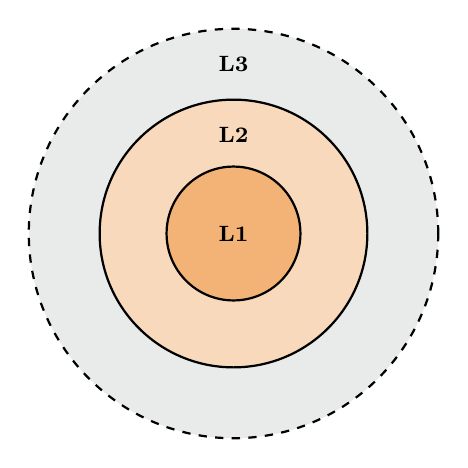
\begin{tikzpicture}[font=\footnotesize]
        \fill[mDarkTeal!10]    (0,0) circle (2.6);
        \fill[mLightBrown!30]  (0,0) circle (1.7);
        \fill[mLightBrown!60]  (0,0) circle (0.85);
        \draw[thick] (0,0) circle (0.85);
        \draw[thick] (0,0) circle (1.7);
        \draw[thick, dashed] (0,0) circle (2.6);

        \node at (0, 0.0)  {\textbf{L1}};
        \node at (0, 1.25) {\textbf{L2}};
        \node at (0, 2.15) {\textbf{L3}};
    \end{tikzpicture}

    \column{0.44\textwidth}
    \small
    \textbf{L1} \emph{what we meant to forget}\\ \footnotesize the unlearned samples themselves

    \vspace{0.4em}
    \small
    \textbf{L2} \emph{collateral forgetting}\\ \footnotesize same cluster $\cdot$ unseen

    \vspace{0.4em}
    \small
    \textbf{L3} \emph{innocent bystanders}\\ \footnotesize other clusters

    \vspace{0.8em}
    \hrule

    \vspace{0.6em}
    \centering
    $r = \dfrac{\text{PPL}_\text{unlearned}}{\text{PPL}_\text{base}}$

    \vspace{0.4em}
    \footnotesize
    take geo-mean per layer\\ $\Rightarrow$ one number for L1 / L2 / L3
    \end{columns}
\end{frame}

% ────────────────────────────────────────────────────────────────────────────
\begin{frame}{Motivation in one line}
    \vfill
    \begin{center}
        \Large
        Switch the forget set $\Rightarrow$ L1 geo differs by \textbf{1.6$\times$}; \emph{log-scale spread} $\approx$ \textbf{1.7$\times$}.
    \end{center}

    \vspace{0.6em}
    \begin{center}
        \normalsize
        Yet each unlearn run costs several GPU-hours.
    \end{center}

    \vspace{1.0em}
    \begin{center}
        \Large
        \alert{Can we predict side-effects without fine-tuning?}
    \end{center}
    \vfill
\end{frame}

% ────────────────────────────────────────────────────────────────────────────
\begin{frame}{How the data is produced: four steps}
    \centering
    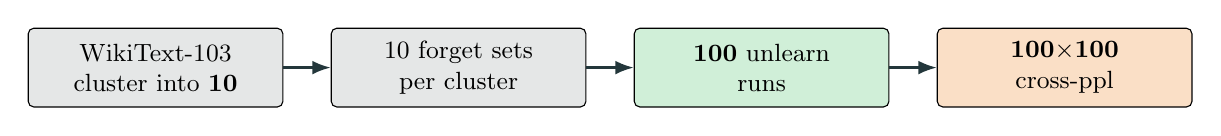
\begin{tikzpicture}[
        box/.style={draw, rounded corners=2pt, align=center,
                    minimum height=10mm, text width=30mm, font=\small},
        arr/.style={-Latex, thick, mDarkTeal},
    ]
        \node[box, fill=mDarkTeal!12] (c) {WikiText-103\\cluster into \textbf{10}};
        \node[box, fill=mDarkTeal!12, right=6mm of c] (t) {10 forget sets\\ per cluster};
        \node[box, fill=mLightGreen!20, right=6mm of t] (u) {\textbf{100} unlearn\\ runs};
        \node[box, fill=mLightBrown!25, right=6mm of u] (m) {\textbf{100$\times$100}\\ cross-ppl};

        \draw[arr] (c) -- (t);
        \draw[arr] (t) -- (u);
        \draw[arr] (u) -- (m);
    \end{tikzpicture}

    \vspace{1.4em}
    \centering
    \large
    Every ckpt eval'd on every triplet $\Rightarrow$ 100$\times$100 matrix
\end{frame}

\begin{frame}{Where L1 / L2 / L3 sit in the cross-matrix}
    \centering
    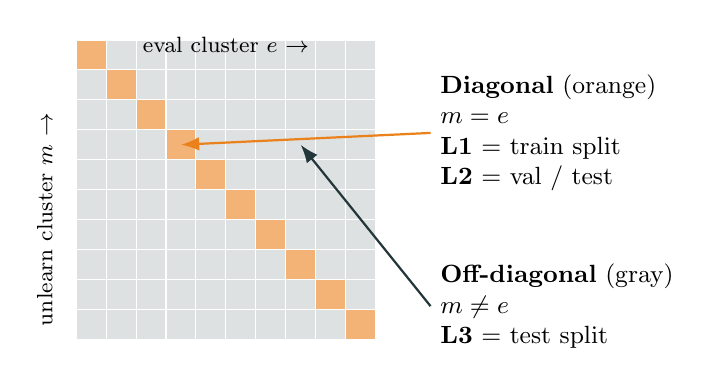
\begin{tikzpicture}[font=\footnotesize]
        \def\s{0.38}
        \foreach \i in {0,...,9} {
            \foreach \j in {0,...,9} {
                \ifnum\i=\j
                    \fill[mLightBrown!60] (\j*\s, -\i*\s) rectangle +(\s,\s);
                \else
                    \fill[mDarkTeal!15] (\j*\s, -\i*\s) rectangle +(\s,\s);
                \fi
                \draw[white, thin] (\j*\s, -\i*\s) rectangle +(\s,\s);
            }
        }
        \node[above] at (10*\s/2, 0.1) {eval cluster $e$ $\to$};
        \node[rotate=90, above] at (-0.18, -10*\s/2) {unlearn cluster $m$ $\to$};

        \node[right, align=left, font=\small] at (10*\s+0.7, -0.8)
            {\textbf{Diagonal} (orange)\\
             $m = e$\\
             \textbf{L1} = train split\\
             \textbf{L2} = val / test};
        \draw[-Latex, thick, mLightBrown] (10*\s+0.7, -0.8) -- (3.0*\s+\s/2, -3.0*\s+\s/2);

        \node[right, align=left, font=\small] at (10*\s+0.7, -3.0)
            {\textbf{Off-diagonal} (gray)\\
             $m \neq e$\\
             \textbf{L3} = test split};
        \draw[-Latex, thick, mDarkTeal] (10*\s+0.7, -3.0) -- (7*\s+\s/2, -3*\s+\s/2);
    \end{tikzpicture}
\end{frame}

% ────────────────────────────────────────────────────────────────────────────
\section{Act I $\cdot$ The three layers are real}

\begin{frame}{Three things this act will show}
    \vspace{0.8em}
    \begin{description}
        \setlength\itemsep{0.8em}
        \item[\alert{C1}] The three layers are \textbf{strictly decreasing} (L1 $>$ L2 $>$ L3), not arbitrary bins.
        \item[\alert{C2}] L3 is \textbf{not zero} --- innocent samples really are hit.
        \item[\alert{C3}] The profile \textbf{varies with the forget set}, so \emph{auditing is worthwhile}.
    \end{description}
\end{frame}

\begin{frame}{C1 + C2: headline numbers}
    \vspace{0.2em}
    \centering
    \small
    $r = \dfrac{\text{PPL}_{\text{unlearned}}}{\text{PPL}_{\text{base}}}$ \;(how many times PPL is raised)\quad
    geo-mean $r = \exp(\overline{\log r})$

    \vspace{0.6em}
    \begin{tabular}{@{}lccc@{}}
        \toprule
        & L1 forget & L2 locality & L3 spillover \\
        \midrule
        geo-mean $r$              & \textbf{1.96$\times$} & \textbf{1.32$\times$} & \textbf{1.19$\times$} \\
        fraction raised ($>1.1\times$) & 100.0\,\%      & 90.8\,\%       & \alert{73.8\,\%} \\
        \bottomrule
    \end{tabular}

    \vspace{1.2em}
    \begin{center}
        \large
        \textbf{C1 holds}: 1.96 $>$ 1.32 $>$ 1.19\\[0.4em]
        \textbf{C2 holds}: L3 still raises \alert{73.8\,\%} of samples
    \end{center}
\end{frame}

\begin{frame}{C1 + C2: one plot}
    \centering
    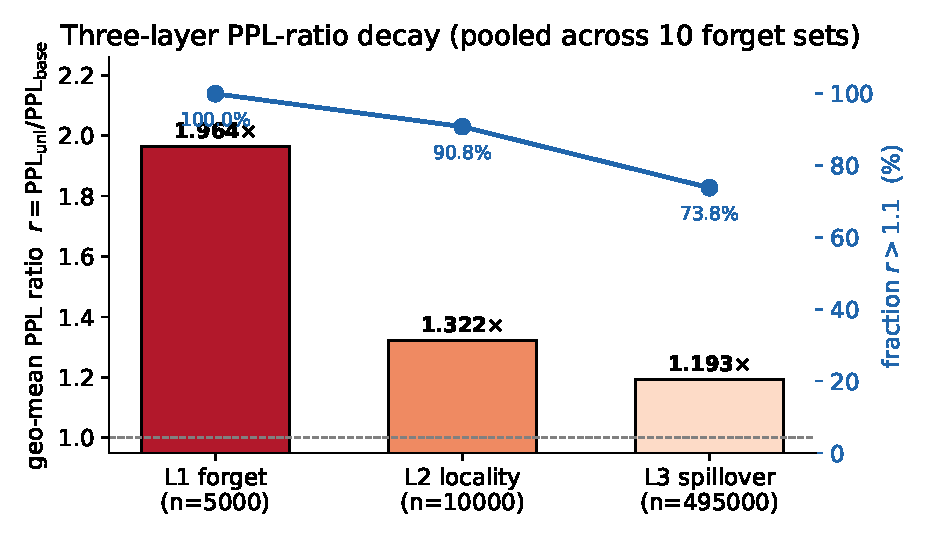
\includegraphics[width=0.82\textwidth]{fig_three_layer_decay.pdf}

    \vspace{0.3em}
    \footnotesize
    Left axis: L1 $>$ L2 $>$ L3\quad|\quad Right axis: L3 still raises \alert{73.8\,\%}.
\end{frame}

\begin{frame}{C3: how much does side-effect vary across forget sets?}
    \centering
    \small
    \begin{tabular}{@{}lccc@{}}
        \toprule
        & L1 & L2 & L3 \\
        \midrule
        mildest triplet (\texttt{029})         & 1.54 & 1.15 & 1.12 \\
        \alert{worst triplet (\texttt{storm 073})} & \alert{\textbf{2.44}} & \alert{\textbf{1.73}} & \alert{\textbf{1.26}} \\
        \midrule
        spread ($n=100$, max / min)    & \textbf{1.59$\times$} & 1.50$\times$ & 1.13$\times$ \\
        \bottomrule
    \end{tabular}

    \vspace{1.2em}
    \begin{center}
        \Large
        Same algorithm, different forget sets $\Rightarrow$ L1 differs by \alert{\textbf{1.6$\times$}}; log-scale spread $\approx 1.7\times$.
    \end{center}

    \vspace{0.4em}
    \begin{center}
        \normalsize
        $\Rightarrow$ The profile is a function of the forget set --- \emph{worth auditing}.
    \end{center}
\end{frame}

\begin{frame}{C3: one plot}
    \centering
    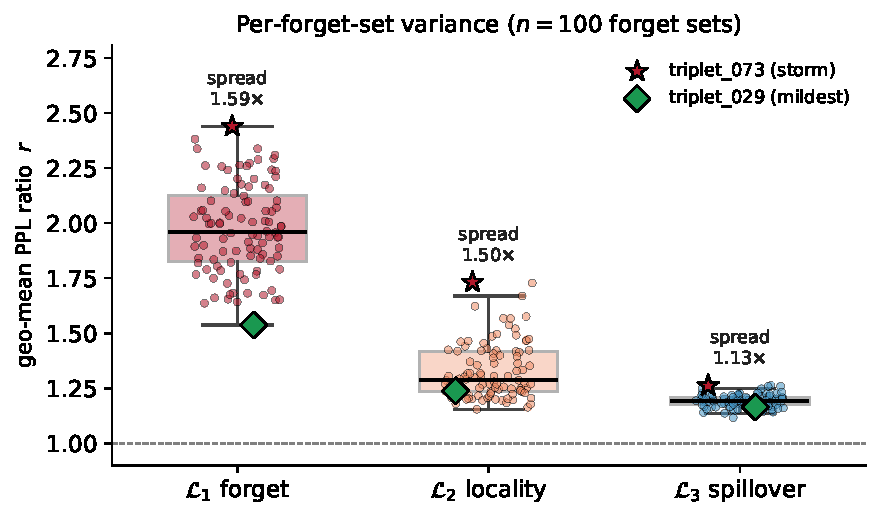
\includegraphics[width=0.88\textwidth]{fig_per_forget_profile.pdf}

    \vspace{0.3em}
    \footnotesize
    Box + jitter ($n=100$); spread reaches $1.59\times$ (L1), $1.50\times$ (L2), $1.13\times$ (L3). \alert{storm} is L1/L2 worst (L3 worst = \texttt{triplet\_072}).
\end{frame}

% ────────────────────────────────────────────────────────────────────────────
\section{Act II $\cdot$ Audit first, then decide}

\begin{frame}{The audit problem: input and output}
    \vspace{0.4em}
    \begin{center}
        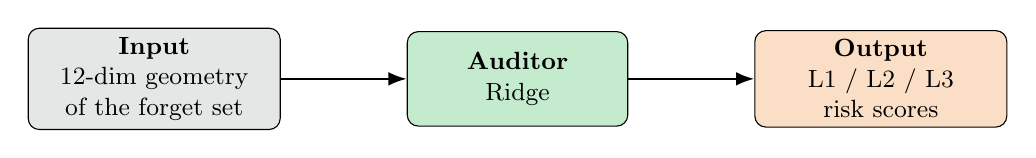
\begin{tikzpicture}[font=\small, node distance=10mm]
            \node[draw, rounded corners, fill=mDarkTeal!12, minimum width=32mm, minimum height=12mm, align=center] (in)
                {\textbf{Input}\\ 12-dim geometry\\ of the forget set};
            \node[draw, rounded corners, fill=mLightGreen!25, right=16mm of in, minimum width=28mm, minimum height=12mm, align=center] (box) {\textbf{Auditor}\\ Ridge};
            \node[draw, rounded corners, fill=mLightBrown!25, right=16mm of box, minimum width=32mm, minimum height=12mm, align=center] (out)
                {\textbf{Output}\\ L1 / L2 / L3\\ risk scores};
            \draw[-Latex, thick] (in) -- (box);
            \draw[-Latex, thick] (box) -- (out);
        \end{tikzpicture}
    \end{center}

    \vspace{0.8em}
    \begin{center}
        \large
        \alert{No evaluation text $\cdot$ no unlearn run}
    \end{center}

    \vspace{0.6em}
    \footnotesize\centering
    12 dims = variance / pairwise similarity / centroid / concentration (effective rank, isotropy).\\
    Leave-One-Out over 100 forget sets.
\end{frame}

\begin{frame}{What are the 12 geometric features?}
    \centering
    \footnotesize
    \begin{tabular}{@{}lll@{}}
        \toprule
        Group & Features (12 total) & Question answered \\
        \midrule
        \textbf{Spread}   & \texttt{emb\_variance\_mean / max}
            & How widely are the 50\\
                          & \texttt{pairwise\_eucl\_mean} & texts spread in embedding space? \\
        \midrule
        \textbf{Similarity} & \texttt{pairwise\_sim\_mean / std / q90}
            & How similar are the texts\\
                            & & to each other? \\
        \midrule
        \textbf{Location / scale} & \texttt{centroid\_norm}
            & How far from the origin\\
                                  & \texttt{emb\_norm\_mean / std} & does the forget set sit? \\
        \midrule
        \textbf{Shape / concentration} & \texttt{effective\_rank}
            & Is the cloud ``a line''\\
                                       & \texttt{isotropy} & or ``a ball''? \\
                                       & \texttt{spread\_over\_centroid} & \\
        \bottomrule
    \end{tabular}

    \vspace{0.8em}
    \begin{center}
        \normalsize
        \textbf{All computed from the 50 embeddings of the forget set itself ---}\\
        no evaluation text, no unlearn run.
    \end{center}
\end{frame}

\begin{frame}{Audit results}
    \centering
    \begin{tabular}{@{}lccc@{}}
        \toprule
        & L1 forget & L2 locality & L3 spillover \\
        \midrule
        $R^2$ (audit / baseline $-0.02$) & \textbf{+0.25} & \textbf{+0.71} & \textbf{+0.22} \\
        MAE (audit / baseline)   & \textbf{0.14} / 0.17 & \textbf{0.05} / 0.11 & \textbf{0.02} / 0.02 \\
        rank Spearman $\rho$     & +0.53 & \textbf{+0.84} & +0.49 \\
        95\% CI ($n_\text{boot}=10$k) & [$+0.37$, $+0.67$] & \textbf{[$+0.76$, $+0.89$]} & [$+0.33$, $+0.63$] \\
        \bottomrule
    \end{tabular}

    \vspace{0.7em}
    \begin{center}
        \Large
        All three layers \emph{significant} (CI exclude 0); \textbf{L2} is strongest
    \end{center}
    \vspace{0.2em}
    \begin{center}
        \normalsize
        Three layers beat LOO-mean baseline; L3 lifted from $R^2=-0.46$ ($n=10$) to $+0.22$ ($n=100$).
    \end{center}

    \vspace{0.2em}
    \footnotesize\centering\itshape
    Held-out: LOO over 100 triplets ($10\text{ clusters} \times 10$), Ridge $\alpha=1$, 12-d forget geometry.
\end{frame}

\begin{frame}{Positioning: a warning tool, not a replacement}
    \centering
    \small
    \begin{tabular}{@{}lll@{}}
        \toprule
         & \textbf{Can} & \textbf{Cannot} \\
        \midrule
        \textbf{Rank}    & tell who is worse (all three $\rho$ exclude 0, L2 $=0.84$) & absolute value \\
        \textbf{Screen}  & red / yellow / green warnings           & score an unlearner \\
        \textbf{Save compute} & 1 s vs. GPU-hours                  & replace the final unlearn \\
        \bottomrule
    \end{tabular}

    \vspace{1.0em}
    \begin{center}
        \Large
        \alert{Auditor = cheap coarse-screening warner}
    \end{center}

    \vspace{0.4em}
    \begin{center}
        \normalsize
        Usage: 100 candidates $\to$ audit rank $\to$ run the top-$k$ for real.\\
        Final verdict still comes from the actual unlearn run.
    \end{center}
\end{frame}

% ────────────────────────────────────────────────────────────────────────────
\section{Discussion}

\begin{frame}{Related Work}
    \small
    Two papers shape how this work is framed.

    \vspace{0.5em}
    \renewcommand{\arraystretch}{1.25}
    \begin{tabular}{@{}p{0.30\textwidth}p{0.33\textwidth}p{0.32\textwidth}@{}}
        \toprule
        \textbf{Paper} & \textbf{What they do} & \textbf{How it shapes us} \\
        \midrule
        \textbf{A Curious Case}\newline\scriptsize Dang+ 2024 \emph{(arXiv 2402.11469)}
            & \emph{Data-first} features of training set $\to$ predict adversarial ASR; 30--193$\times$ faster than model-first
            & Same paradigm transferred: forget-set 12-d geometry $\to$ predict $L_1$/$L_2$/$L_3$ corruption without running unlearn \\
        \midrule
        \textbf{Probing Knowledge Holes}\newline\scriptsize Ko+ 2025 \emph{(arXiv 2511.00030)}
            & Unlearn leaves \emph{adjacent / latent knowledge holes} that standard utility benchmarks miss; they \emph{probe} post-unlearn
            & Exactly the phenomenon our $L_2$ locality + $L_3$ spillover quantify --- but we \emph{audit pre-unlearn}, not probe after \\
        \bottomrule
    \end{tabular}

    \vspace{0.5em}
    \footnotesize\itshape
    One-liner: Dang+ taught us \emph{how to predict from data side}; Ko+ told us \emph{what to predict}.
\end{frame}

\begin{frame}{Limitations}
    \vspace{0.3em}
    \begin{center}
        \large
        Four ``singles''
    \end{center}

    \vspace{0.6em}
    \begin{itemize}
        \setlength\itemsep{0.6em}
        \item single base model (Llama-3.1-8B-Instruct)
        \item single unlearner (GradAscent)
        \item $n = 100$ forget sets (all three CIs exclude 0; L3 still the weakest $R^2$)
        \item single metric: PPL ($\neq$ QA accuracy)
    \end{itemize}
\end{frame}


\begin{frame}{Paper positioning}
    \begin{center}
        \large
        \emph{From Three-Layer Corruption to Forget-Set Audit\\ in LLM Unlearning.}
    \end{center}

    \vspace{0.8em}
    \textbf{Three selling points}
    \begin{enumerate}
        \item three-layer view + L3 raises 73.8\,\% of cross-topic text $\Rightarrow$ spillover \emph{non-negligible}
        \item benchmarking $\to$ \textbf{forget-set audit} perspective shift
        \item geometry alone ranks corruption --- L2 $R^2=+0.71$, L3 lifts to $+0.22$ at $n=100$, all $\rho$ CIs exclude 0
    \end{enumerate}

    \vspace{0.6em}
    \begin{center}
        \small
        \textbf{Status}: $n{=}100$ \checkmark\quad \textbf{Next}: NPO / GradDiff \;+\; QA-label metric $\Rightarrow$ NeurIPS / ICML
    \end{center}
\end{frame}

\end{document}
